%% LyX 2.0.3 created this file.  For more info, see http://www.lyx.org/.
%% Do not edit unless you really know what you are doing.
\documentclass[english,11pt]{article}
\usepackage[T1]{fontenc}
\usepackage[latin9]{inputenc}
\usepackage{geometry}
\geometry{verbose,tmargin=1in,bmargin=1in,lmargin=1in,rmargin=1in}
\setlength{\parskip}{\medskipamount}
\setlength{\parindent}{0pt}
\usepackage{babel}
\usepackage{float}
\usepackage{rotfloat}
\usepackage{amsthm}
\usepackage{amsmath}
\usepackage{amssymb}
\usepackage{graphicx}
\usepackage{setspace}
\doublespacing
\usepackage[unicode=true,pdfusetitle,
 bookmarks=true,bookmarksnumbered=false,bookmarksopen=false,
 breaklinks=false,pdfborder={0 0 0},backref=false,colorlinks=false]
 {hyperref}
\usepackage{breakurl}

\makeatletter
%%%%%%%%%%%%%%%%%%%%%%%%%%%%%% Textclass specific LaTeX commands.
\numberwithin{equation}{section}
\numberwithin{figure}{section}
\theoremstyle{plain}
\newtheorem{thm}{\protect\theoremname}
  \theoremstyle{definition}
  \newtheorem{defn}[thm]{\protect\definitionname}
  \theoremstyle{plain}
  \newtheorem{conjecture}[thm]{\protect\conjecturename}
  \theoremstyle{plain}
  \newtheorem{lem}[thm]{\protect\lemmaname}
  \theoremstyle{plain}
  \newtheorem{cor}[thm]{\protect\corollaryname}
  \theoremstyle{plain}
  \newtheorem{prop}[thm]{\protect\propositionname}

\@ifundefined{date}{}{\date{}}
%%%%%%%%%%%%%%%%%%%%%%%%%%%%%% User specified LaTeX commands.
\usepackage{tikz}
\usepackage{pgfplots}
\usetikzlibrary{arrows,automata,shapes,chains,positioning}

\usepackage{amsfonts}

% redefine ensuremath to put a space behind it
% this fixes broken LyX behavior that removes spaces behind it sometimes
\usepackage{xspace} % conditional spaceing
\let\Oldensuremath\ensuremath
\renewcommand{\ensuremath}[1]{\Oldensuremath{#1}\xspace}

\makeatother

  \providecommand{\conjecturename}{Conjecture}
  \providecommand{\corollaryname}{Corollary}
  \providecommand{\definitionname}{Definition}
  \providecommand{\lemmaname}{Lemma}
  \providecommand{\propositionname}{Proposition}
\providecommand{\theoremname}{Theorem}

\begin{document}


\global\long\def\Sym{\operatorname{Sym}}


\global\long\def\Aut{\operatorname{Aut}}


\global\long\def\Ker{\operatorname{Ker}}


\global\long\def\Img{\operatorname{Im}}


\global\long\def\Sep{\operatorname{Sep}}


\global\long\def\powerset{\operatorname{\mathcal{P}}}




\global\long\def\functionclass#1{\mathcal{#1}}


\global\long\def\FP{\functionclass{FP}}




\global\long\def\complexityclass#1{\mathrm{#1}}


\global\long\def\DTIME{\complexityclass{DTIME}}
\global\long\def\NTIME{\complexityclass{NTIME}}
\global\long\def\coNTIME{\complexityclass{coNTIME}}


\global\long\def\P{\complexityclass P}
\global\long\def\NP{\complexityclass{NP}}
\global\long\def\coNP{\complexityclass{coNP}}


\global\long\def\UP{\complexityclass{UP}}


\global\long\def\E{\complexityclass E}
\global\long\def\NE{\complexityclass{NE}}
\global\long\def\coNE{\complexityclass{coNE}}


\global\long\def\EE{\complexityclass{EE}}
\global\long\def\NEE{\complexityclass{NEE}}
\global\long\def\coNEE{\complexityclass{coNEE}}


\global\long\def\EEE{\complexityclass{EEE}}
\global\long\def\NEEE{\complexityclass{NEEE}}
\global\long\def\coNEEE{\complexityclass{coNEEE}}


\global\long\def\EXP{\complexityclass{EXP}}
\global\long\def\NEXP{\complexityclass{NEXP}}
\global\long\def\coNEXP{\complexityclass{coNEXP}}


\global\long\def\DisjNP{\complexityclass{DisjNP}}


\global\long\def\SPARSE{\complexityclass{SPARSE}}


\global\long\def\degree{\operatorname{d}}


\global\long\def\GI{\complexityclass{GI}}
\global\long\def\GNI{\complexityclass{GNI}}


\global\long\def\AM{\complexityclass{AM}}
\global\long\def\coAM{\complexityclass{coAM}}


\global\long\def\Few{\complexityclass{Few}}


\global\long\def\FewP{\complexityclass{FewP}}




\global\long\def\redmo{\leq_{m}^{p}}
\global\long\def\equivmo{\equiv_{m}^{p}}


\global\long\def\redt{\leq_{T}^{p}}
\global\long\def\equivt{\equiv_{T}^{p}}


\global\long\def\redr{\leq_{r}}
\global\long\def\nredr{\nleq_{r}}




\global\long\def\predmo{\leq_{m}^{pp}}
\global\long\def\pequivmo{\equiv_{m}^{pp}}


\global\long\def\predsmo{\leq_{sm}^{pp}}
\global\long\def\pequivsmo{\equiv_{sm}^{pp}}


\global\long\def\predt{\leq_{T}^{pp}}
\global\long\def\pequivt{\equiv_{T}^{pp}}


\global\long\def\predunimo{\leq_{um}^{pp}}
\global\long\def\pequivunimo{\equiv_{um}^{pp}}


\global\long\def\predunit{\leq_{uT}^{pp}}
\global\long\def\pequivunit{\equiv_{uT}^{pp}}


\global\long\def\predr{\leq_{r}^{pp}}
\global\long\def\pequivr{\equiv_{r}^{pp}}




\global\long\def\simp{\leq_{p}}




\global\long\def\lang#1{\mathrm{#1}}


\global\long\def\SAT{\lang{SAT}}
\global\long\def\SATstar{\lang{SAT}^{*}}


\global\long\def\REF{\lang{REF}}


\global\long\def\TAUT{\lang{TAUT}}


\global\long\def\TALLY{\lang{TALLY}}




\global\long\def\true{\text{true}}
\global\long\def\false{\text{false}}




\newcommand{\keyreturn}{return}

\pagebreak{}

\vspace*{.5in}

\noindent \begin{center}
\textbf{\LARGE Survey of Disjoint $\NP$-Pairs and Propositional Proof
Systems }
\par\end{center}{\LARGE \par}

\noindent \begin{center}
by
\par\end{center}

\noindent \begin{center}
{\LARGE Nils Wisiol}
\par\end{center}{\LARGE \par}

\noindent \begin{center}
September, 1st 2014
\par\end{center}

\vfill

\noindent \begin{center}
A thesis submitted to the Faculty of the Graduate School of the University
at Buffalo, State University of New York in partial fulfillment of
the requirements for the degree of
\par\end{center}

\noindent \begin{center}
{\LARGE Master of Science}
\par\end{center}{\LARGE \par}

\noindent \begin{center}
Department of Computer Science and Engineering
\par\end{center}

\thispagestyle{empty}

\newpage{}

\renewcommand{\thepage}{\roman{page}}

\vspace*{1in}\vfill

\noindent \begin{center}
Copyright by\\
Nils Wisiol\\
2014
\par\end{center}

\newpage{}

\vspace*{2in}

\begin{singlespace}
\noindent \begin{center}
\emph{I wish to thank my advisors Alan Selman (University at Buffalo)
and Christian Gla�er (Universit�t W�rzburg, Germany), committee member
Ken Regan and my friends and fellow students Andrew Hughes and Michael
Wehar for their great support, patience, knowledge and comments.}
\par\end{center}
\end{singlespace}

\begin{singlespace}
\noindent \newpage{}
\end{singlespace}

\tableofcontents{}

\newpage{}

Abstract 300-400 words

\newpage{}

\setcounter{page}{1}

\renewcommand{\thepage}{\arabic{page}}


\section{Introduction\label{sec:Introduction}}

This thesis aims at readers that do not have a strong background in
the theories of propositional proof systems and disjoint $\NP$ pairs.
It surveys important results from both and points out important connections
in between these two theories. Core of the thesis is the implication
chart in Figure \ref{fig:implication-chart}, that summarizes virtually
all results mentioned in this thesis.

In Section \ref{sec:Preliminaries} is split into two pieces. In \ref{sub:Disjoint--Pairs},
we introduce the reader to the theory of disjoint $\NP$-pairs based
on the notion of promise problems. In \ref{sub:Propositional-Proof-Systems},
we familiarize ourselves with propositional proof systems. Both introductions
contain history, motivation and notions of the theories. In Section
\ref{sub:Propositional-Proof-Systems}, we give basic results and
proofs that help the reader understanding the introduced notions.
Readers familiar with notions from both fields can safely skip this
Section.

Section \ref{sec:Disjoint--Pairs} covers important results from the
field of disjoint $\NP$-pairs. We will study the earlier introduced
reducibility of pairs in greater detail. It turns out that various
definitions of reducibility available in the literature are equivalent.
Subsequently, we study refinements of the ESY-conjecture and connections
to open questions of complexity class separation.

Greater details of the theory of propositional proof systems will
be covered in Section \ref{sec:Propositional-Proof-Systems}. We will
justify the motivation to study proof systems by establishing an equivalent
formulation of $\NP=\coNP$, before we look into sufficient and necessary
conditions for their existence. These conditions will lay the foundation
for the study of different oracles in Section \ref{sec:Relativized-Worlds}.

Section \ref{sec:Canonical-Disjoint--pairs} finally covers the connection
in between both theories that was discovered by Razborov. It presents
a proof for Razborov's theorem that uses the notion of complexity
theory.

We also take a look on relativized worlds in Section \ref{sec:Relativized-Worlds}.
We point the reader to oracles relative to which optimal proof systems
exist respectively do not exist. Section \ref{sub:Converse-of-Razborov}
studies the converse of Razborov's theorem, for which we know oracles
relative to which it holds, and relative to which it does not hold.
Finally we refer the reader to a oracle that separates different refinements
of the ESY-conjecture from each other.

We conclude the thesis with a summary of open questions and future
work on the field in Section \ref{sec:Conclusion}.

\begin{sidewaysfigure}
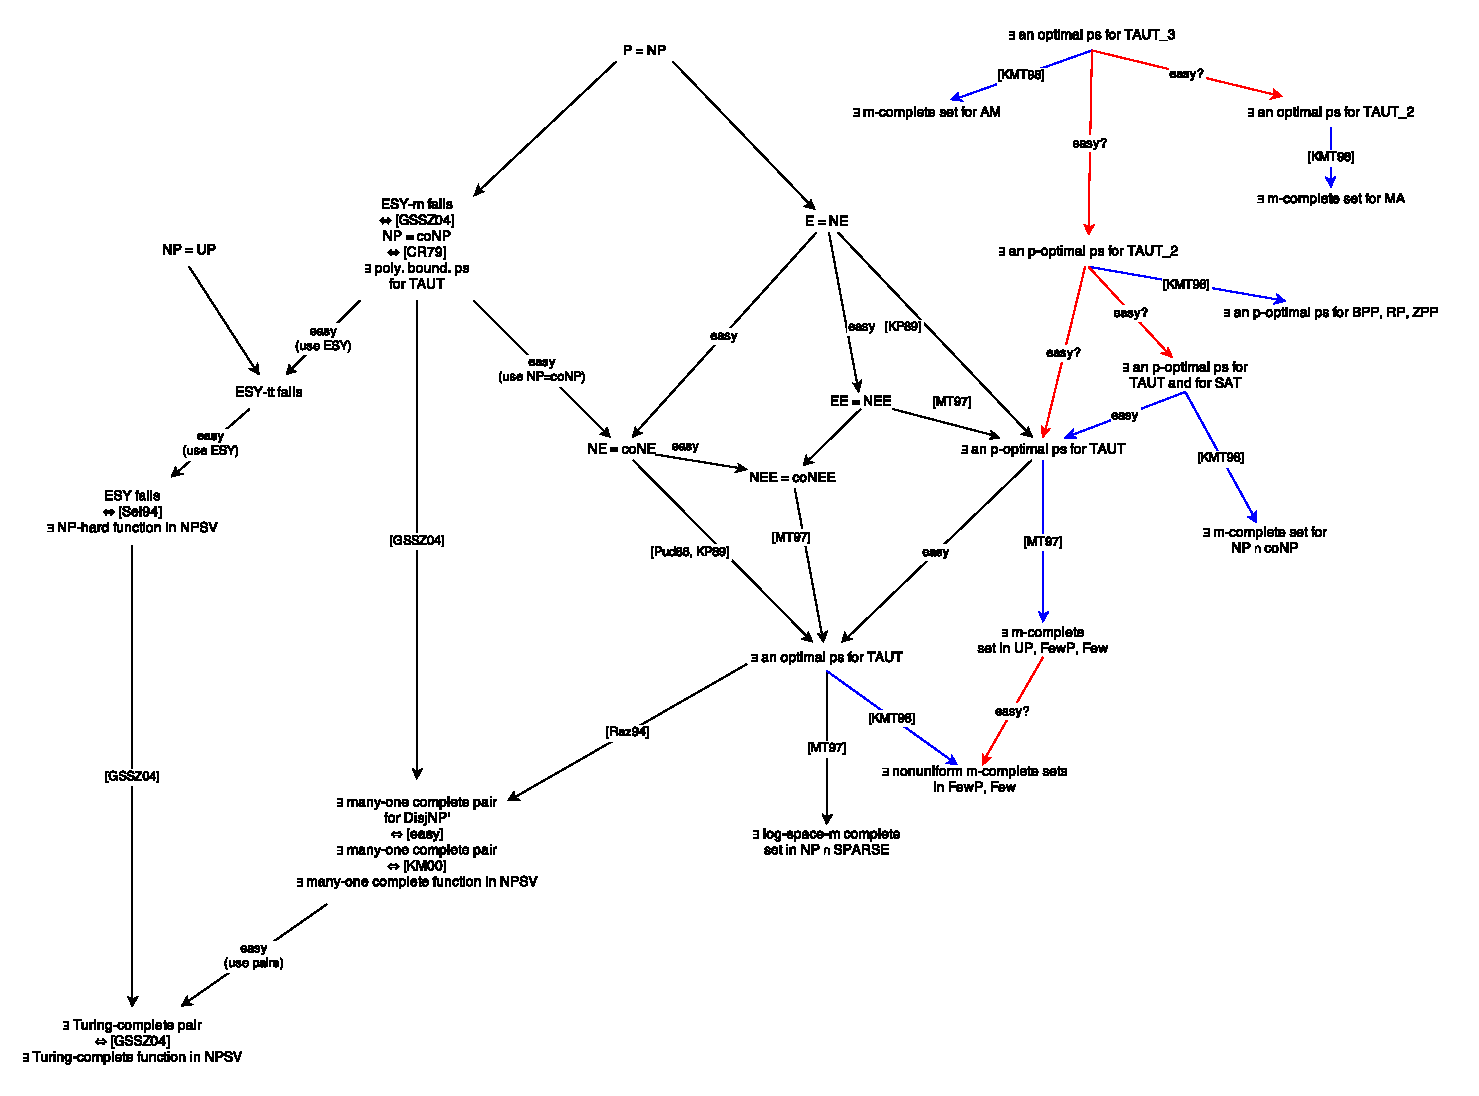
\includegraphics[width=1\textwidth]{implicationchart}

\caption{Known Implications for proof systems, disjoint pairs and the ESY conjecture
\label{fig:implication-chart}}
\end{sidewaysfigure}
\newpage{}


\section{Preliminaries\label{sec:Preliminaries}}


\subsection{Disjoint $\NP$-Pairs\label{sub:Disjoint--Pairs}}

The study of disjoint $\NP$-pairs originates in the study of public
key crypto systems (PKCS). The interest in secure PKCS is fundamental
to everyday life as well as to academia, as provably hard-to-crack
PKCS would imply $\NP\neq\P$.

To study the hardness of PKCS, Even, Selman and Yacobi used the notion
of \emph{promise problems} rather than decision problems to model
the problem of cracking a PKCS \cite{journals/iandc/EvenSY84}. In
fact, promise problems are a generalization of decision problems.
A machine working on a promise problem is not only given an input,
but also a promise that for this input, a certain condition holds.
The machine \emph{solves} the problem, if it gives the right answer
on all inputs for which the promise holds. If the promised condition
does in fact not hold for a given input, then the machine can act
arbitrarily.

We can define promise problems more formally, following Goldreich's
survey \cite{DBLP:journals/eccc/ECCC-TR05-018}: A promise problem
is a partition of the set of all strings into three subsets:
\begin{enumerate}
\item The set of strings representing Yes-Instances,
\item the set of strings representing No-Instances, and
\item the set of disallowed strings.
\end{enumerate}
We can write this partition as a pair of two disjoint sets $(A,B)$,
where $A$ and $B$ represent Yes- and No-Instances, and the set of
disallowed strings is $\overline{A\cup B}$. The \emph{promise} in
this setting is that a given input string either belongs to $A$ or
$B$. If $\overline{A\cup B}=\emptyset$, then the promise problem
has no disallowed strings and thus no promise, it is in fact a decision
problem.%
\footnote{Even, Selman and Yacobi \cite{journals/iandc/EvenSY84} used a pair
$(Q,R)$ to represent promise problems, where $Q$ is a predicate
true for all \emph{allowed }strings (the \emph{promise}) and $R$
is a predicate true for all Yes-Instances (the \emph{property}). This
relates with Goldreich's definition as follows: 
\begin{eqnarray*}
A\cup B & = & \{w\in\Sigma^{*}\mid Q(w)\}\\
A & = & \{w\in\Sigma^{*}\mid Q(w)\wedge R(w)\}\\
B & = & \{w\in\Sigma^{*}\mid Q(w)\wedge\neg R(w)\}
\end{eqnarray*}
%
}

Using this notation, we can define a promise problem that captures
the hardness of cracking the PKCS, that is, captures the hardness
of finding the plain text to a given cipher text $C$ and public key
$K$. To crack the crypto system, we will conduct a binary search
among all strings up to a reasonable length. The scope for the binary
search is limited, as the length of the plain text is polynomial in
the length of the cipher text. Notice that this notion captures the
hardness to crack \emph{every} cipher text in a PKCS. While we can
conclude cryptographic insecureness from an easy cracking problem,
a hard cracking problem does not imply cryptographic security, as
a subset of cipher texts may be still easy to crack. 

The promise problem is defined as follows:
\begin{enumerate}
\item The set of Yes-Instances will be the set of strings $\langle M',C,K\rangle$
for which there exists a message $M$, $M\leq M'$, such that $M$
encrypted with $K$ yields cipher text $C$.
\item The set of No-Instances will be the set of strings $\langle M',C,K\rangle$
for which there exists a message $M$, $M>M'$, such that $M$ encrypted
with $K$ yields cipher text $C$.
\item The set of disallowed strings will be all triples $\langle M',C,K\rangle$
such that for all plain texts $M$, encryption with $K$ does not
yield $C$.
\end{enumerate}
With a machine solving this promise problem, we can find the plain
text to any given $C$ and $K$ by binary search over all messages
$M'$. Thus, the runtime of cracking the PKCS is within a logarithmic
factor of the runtime of the machine solving the promise problem.
Therefore, we consider the hardness of the promise problem itself
as a good measurement for the hardness of the cracking problem.

But why not model the cracking problem as a decision problem? To see
why a simple decision problem does not capture the cracking problem
correctly, assume we have a PKCS such that the \emph{decision }problem
$A$ is not efficiently computable. However, if there is an algorithm
efficiently solving the promise problem $(A,B)$, the crypto system
would still be easy to crack. On the other hand, if the promise problem
is hard, the decision problem will also be.

To capture the situation where we have a hard decision problem, but
an easy promise problem, we call a set $S$ for which $A\subseteq S$
and $B\subseteq\overline{S}$ \emph{a separator.} Let the set $\Sep(A,B)$
denote the set of all separators for a given pair $(A,B)$. A pair
$(A,B)$ that has no polynomial-time decidable set in $\Sep(A,B)$
is called \emph{$\P$-inseparable}, otherwise it is called \emph{$\P$-separable}.

The interesting class of promise problems $(A,B)$ is the class with
promises that are not polynomial-time decidable. In the contrary case
where $A\cup B$ is efficiently computable, deciding the promise problem
$(A,B)$ is polynomial-time equivalent to solving the decision problems
$A$ or $B$.

Assigning a hardness to PKCS immediately calls for a notion that compares
the hardness of two promise problems. Following Grollmann and Selman
\cite{journals/siamcomp/GrollmannS88}, we use the following reductions
for promise problems that naturally arise from the reductions of languages.
\begin{defn}
\label{def:pair-reduction}
\begin{enumerate}
\item A promise problem $(A,B)$ is \emph{many-one-reducible in polynomial
time} to $(C,D)$, $(A,B)\predmo(C,D)$, if for every separator $T\in\Sep(C,D)$,
there exists a separator $S\in\Sep(A,B)$ such that $S\redmo T$.
\item A promise problem $(A,B)$ is \emph{many-one-reducible in polynomial
time} to $(C,D)$, $(A,B)\predt(C,D)$, if for every separator $T\in\Sep(C,D)$,
there exists a separator $S\in\Sep(A,B)$ such that $S\redt T$.
\item As a generalization of the previous two, we define a promise problem
$(A,B)$ to be $r$-\emph{reducible} to $(C,D)$, $(A,B)\predr(C,D)$,
if for every separator $T\in\Sep(C,D)$, there exists a separator
$S\in\Sep(A,B)$ such that $S\redr T$.
\item A promise problem $(A,B)$ is $\NP$-hard, if for every Turing machine
$M$ that solves $(A,B)$, the language accepted by $M$ is $\NP$-hard.
\end{enumerate}
\end{defn}
A promise problem $(A,B)$ with $A,B\in\NP$ is a \emph{disjoint $\NP$-pair}.
We define $\DisjNP$ to be the set of all disjoint $\NP$-pairs. For
this class, we define completeness:
\begin{defn}

\begin{enumerate}
\item A disjoint $\NP$-pair $(A,B)$ is $\predmo$-complete, if for every
$(C,D)\in\DisjNP$ we have $(C,D)\predmo(A,B)$.
\item A disjoint $\NP$-pair $(A,B)$ is $\predt$-complete, if for every
$(C,D)\in\DisjNP$ we have $(C,D)\redt(A,B)$.
\end{enumerate}
\end{defn}
We define $\predr$-completeness analogously.

Evan, Selman and Yacobi found out that if disjoint $\NP$-pairs that
are $\NP$-hard do not exist, then there is exist no PKCS with $\NP$-hard
cracking problems. This gives additional motivation for the study
of disjoint $\NP$-pairs, which also arise from the study of recursively
inseparable sets. 

The assertion that there are no disjoint $\NP$-pairs that are $\NP$-hard
to solve has many more consequences and has been studied well since
it was formulated as a conjecture by Even, Selman, and Yacobi \cite{journals/iandc/EvenSY84}.
\begin{conjecture}[ESY]
 For every pair of disjoint sets in $\NP$, there is a separator
that is not Turing-hard for $\NP$. \cite{journals/iandc/EvenSY84} 
\end{conjecture}
If the conjecture holds, then no PKCS is $\NP$-hard to crack. The
following refined version of the ESY-conjecture can be proven to be
equivalent to $\NP\neq\coNP$, see Theorem \ref{thm:equiv-esymfails-np=00003Dconp-polyboundpps}.
\begin{conjecture}[ESY-m]
 For every pair of disjoint sets in $\NP$, there is a separator
that is not many-one-hard for $\NP$. \cite{conf/icalp/HughesPRS12} 
\end{conjecture}
We will study the consequences of the ESY-conjectures in Section \ref{sub:ESY-conjectures}.


\subsection{Propositional Proof Systems\label{sub:Propositional-Proof-Systems}}

A propositional proof system is a fast method of verifying proofs.

To give an example, we will have a look at the \emph{resolution principle},
which was introduced by Robinson \cite{journals/jacm/Robinson65}.
Consider a boolean formula $\varphi$ in conjunctive normal form.
If $\varphi$ is not satisfiable, the resolution principle provides
a way to find a proof for this fact. To find a proof, the resolution
principle iteratively combines two existing clauses into a new and
shorter clause with equivalent truth value. Robinson showed that the
resolution principle yields the empty clause eventually for any unsatisfiable
formula, and any formula for which the principle yields the empty
clause is unsatisfiable:
\begin{thm}[Resolution Theorem \cite{journals/jacm/Robinson65}]
\label{thm:resolution-theorem} For a formula $\varphi$ in conjunctive
normal form, the resolution principle yields the empty clause if and
only if $\varphi$ is not satisfiable.
\end{thm}
As we can see from the way resolution works, there are exponentially
many options how to combine the clauses, and not every sequence of
combinations will yield the empty clause. Hence, it is hard to find
a sequence of combinations that derive the empty clause. By Theorem
\ref{thm:resolution-theorem}, this sequence exists if and only if
the formula is unsatisfiable. As opposed to finding a sequence, given
a sequence of combinations, we can easily check if this sequence derives
the empty clause.

Using formal terms, let $f$ be defined by
\[
f(\langle\varphi,w\rangle)=\begin{cases}
\neg\varphi & \text{if combination sequence \ensuremath{w}applied to \ensuremath{\varphi}yields the empty clause,}\\
\perp & \text{otherwise.}
\end{cases}
\]
Intuitively, $f$ is polynomial-time computable. By the Resolution
Theorem, $f$ only outputs tautologies, and for every tautology $\neg\varphi$,
there is an input $\langle\varphi,w\rangle$ such that $f(\langle\varphi,w\rangle)=\neg\varphi$. 

Given a combination sequence $w$ that yields the empty clause for
$\varphi$, the function $f$ provides a fast way to verify $\neg\varphi$
is a tautology. We thus call $f$ a propositional proof system, and
we call $\langle\varphi,w\rangle$ a $f$-proof for $\neg\varphi$.
\begin{defn}
A polynomial-time computable function $f$ that is onto the set of
tautologies is called a \emph{propositional proof system} or \emph{proof
system}. For any $w$, we say $w$ is a \emph{$f$-proof for $x$}
if $f(w)=x$. If there is a polynomial $p$, such that for all $x$,
and all $f$-proofs $w$ of $x$, we have $|w|\leq p(|x|)$, then
$f$ is \emph{polynomially-bounded}.
\end{defn}


Cook and Reckhow started a line of research \cite{journals/jsyml/CookR79}
that tries to investigate what the length of the shortest proof of
a propositional tautology relative to the length of the tautology
is. The interest in the length of the proof is motivated by the fact
that the existence of polynomial-length proofs for all tautologies
characterizes the question of whether $\NP=\coNP$. (A fact we will
prove in Section \ref{sec:Propositional-Proof-Systems}.) However,
no known proof system could be proven to have proofs with length bounded
by a polynomial. To tackle the problem, Cook and Reckhow introduced
the notion of simulation of proof systems.
\begin{defn}
Let $f$ and $g$ be proof systems. We say $f$ \emph{simulates} $g$,
if there is a function $h$ such that for all $w$, it holds $f(h(w))=g(w)$
and $|h(w)|\leq p(|w|)$. If $h$ is polynomial-time computable, we
say $f$ \emph{p-simulates} $g$. A proof system that simulates (p-simulates)
every other proof system is called \emph{optimal} (\emph{p-optimal}).
\end{defn}
An more intuitive (and informal) way to give a definition for ``$f$
simulates $g$'' is to say that for every tautology $\varphi$, the
$f$-proof for $\varphi$ is at most polynomially longer than the
$g$-proof of $\varphi$. An optimal proof system then has the shortest
proofs for tautologies among all proof systems, within a polynomial
factor.

However, it is not only unknown whether polynomially-bounded proof
systems exist, it is also unknown if optimal or even p-optimal proof
systems exist. To study the existence of optimal and p-optimal proof
systems, we will therefore study sufficient conditions and implications
in Section \ref{sec:Propositional-Proof-Systems}. To become familiar
with the notions, we present a strong sufficient condition for the
existence of optimal proof systems:
\begin{thm}
\label{thm:np-eq-conp-implies-optimalpps}If $\NP=\coNP$, then there
is an optimal proof system.\end{thm}
\begin{proof}
Let $N$ be a $\NP$-machine deciding $\TAUT\in\coNP$. We define
$f$ by 
\[
f(\langle i,x\rangle)=\begin{cases}
x & \text{if \ensuremath{N}accepts \ensuremath{w}along path \ensuremath{i},}\\
\perp & \text{otherwise}.
\end{cases}
\]
Notice, a proof system does not have to be a total function. By definition,
$f$ outputs only tautologies, and for every tautology there is an
accepting path of $N$, so $f$ is onto $\TAUT$.

To see $f$ is optimal, let $f'$ be an arbitrary proof system. There
is a function $g$ mapping each tautology $w$ to an accepting path
$i$ of $N$. Notice, $g$ might not by polynomial-time computable,
but is polynomially length bounded. Let now $w$ be a $f'$-proof
for $x$. With $g$, we can translate $w$ into $\langle g(w),f'(w)\rangle$,
which is a $f$-proof for $x$.
\end{proof}
As we will see in Section \ref{sec:Propositional-Proof-Systems},
the existence of both optimal and p-optimal proof systems can be proven
under much weaker hypotheses.


\section{Disjoint $\NP$-Pairs\label{sec:Disjoint--Pairs}}

One of the most interesting open questions about disjoint $\NP$-pairs
is whether there are complete pairs, either $\predmo$- or $\predt$-complete.
A proof of the non-existence of either one would prove $\NP\neq\coNP$
and $\P\neq\NP$, but we can also relate complete pairs to propositional
proof systems. Using the ESY-conjectures, we can also relate disjoint
$\NP$-pairs to the $\NP$ vs. $\coNP$ questions.


\subsection{Reducibility of disjoint pairs\label{sub:Reducibility-of-disjoint}}

In the literature exist several different definitions for the reducibility
of pairs. Notice that results from this section apply to all disjoint
pairs $(A,B)$; the sets are \emph{not} required to be in $\NP$.
Additionally to the definition \ref{def:pair-reduction} given above
in the introduction, Grollmann and Selman \cite{journals/siamcomp/GrollmannS88}
also define the notion of \emph{uniform} reductions of pairs:
\begin{defn}
Let $(A,B)$ and $(C,D)$ be disjoint pairs. \label{def:uniform-pair-reduction}
\begin{enumerate}
\item $(A,B)$ is \emph{uniformly many-one reducible in polynomial time}
to $(C,D)$, $(A,B)\predunimo(C,D)$, if there exists a polynomial-time
computable function $f$ such that for every separator $T\in\Sep(C,D)$,
there exists a separator $S\in\Sep(A,B)$ such that $S\redmo T$ via
$f$.
\item $(A,B)$ is \emph{uniformly Turing reducible in polynomial time} to
$(C,D)$, $(A,B)\predunit(C,D)$, if there exists a polynomial-time
oracle Turing machine $M$ such that for every separator $T\in\Sep(C,D)$,
there exists a separator $S\in\Sep(A,B)$ such that $S\redt T$ via
$M$.
\end{enumerate}
\end{defn}
Notice that this definition requires that all separators reduce via
the same function or machine. Definition \ref{def:pair-reduction},
the definition of nonuniform reducibility, does not require this.
In spite of this, surprisingly, it turns out that the uniform and
nonuniform variant of the definition are equivalent.

Razborov uses yet another definition of many-one reducibility of pairs:
\begin{defn}
Let $(A,B)$ and $(C,D)$ be disjoint pairs. $(A,B)$ is Razborov
reducible%
\footnote{Razborov reducible is not a term commonly used in the literature.
We will use it only to prove equivalence to many-one reducibility
in Lemma \ref{lem:reducibilities}.%
} to $(C,D)$, if there exists a polynomial-time computable function
$\lambda$ such that $\lambda(A)\subseteq C$ and $\lambda(B)\subseteq D$.
\end{defn}
It turns out that this is equivalent to the many-one reducibility
defined above as well. As a summary of all these definitions, we obtain
the following lemma. A comprehensive proof of it can be found Gla�er,
Selman, Sengupta and Zhang \cite[Theorems 2.8, 2.10, 2.14]{journals/eccc/ECCC-TR03-011}.
\begin{lem}
\label{lem:reducibilities}Let $(A,B)$ and $(C,D)$ be disjoint pairs.
Then the following assertions are equivalent:
\begin{enumerate}
\item $(A,B)\predmo(C,D)$
\item $(A,B)\predunimo(C,D)$
\item There exists a polynomial-time computable function $\lambda$ such
that $\lambda(A)\subseteq C$ and $\lambda(B)\subseteq D$.
\end{enumerate}
The assertions above imply the following equivalent statements:
\begin{enumerate}
\item $(A,B)\predt(C,D)$
\item $(A,B)\predunit(C,D)$
\end{enumerate}
\end{lem}
Therefore, for the rest of this thesis, we will only use many-one
and Turing reducibility.


\subsection{ESY-conjectures\label{sub:ESY-conjectures}}

The original ESY-conjecture \cite{journals/iandc/EvenSY84} is that
for every pair of disjoint sets in $\NP$, there is a separator that
is not Turing-hard for $\NP$. This can easily be refined by using
many-one hardness instead of Turing-hardness.
\begin{defn}
For a reduction $r$, we define the ESY-$r$ conjecture as follows:
For every pair of disjoints sets in $\NP$, there is a separator that
is not $r$-hard for $\NP$,
\[
\forall_{(A,B)\in\DisjNP}\exists_{S\in\Sep(A,B)}\exists_{L\in\NP}L\nredr S.
\]
Notice, ESY-$T$ is the original ESY conjecture.
\end{defn}
The negation of the ESY-$r$ conjecture is 
\[
\exists_{(A,B)\in\DisjNP}\forall_{S\in\Sep(A,B)}\forall_{L\in\NP}L\redr S,
\]
that is, there exists a disjoint $\NP$-pair $(A,B)$ such that all
separators are $r$-hard for $\NP$. Since the different reductions
imply each other, we obtain a implication chain of ESY-conjectures:
\begin{lem}
Each item implies the following item in the list:
\begin{enumerate}
\item ESY-$m$ does not hold.
\item ESY-$tt$ does not hold.
\item ESY-$T$ (the original ESY conjecture) does not hold.
\end{enumerate}
\end{lem}
This list can, of course, be extended to a lot more reductions of
languages. In this thesis, we mention these specific reductions because
there are known results that relate to these assertions.

The ESY-conjectures immediately relate to the existence of complete
pairs, as we can see from the negated ESY-$r$ statement.
\begin{thm}
If ESY-$r$ does not hold, then there exists a $r$-complete disjoint
$\NP$ pair.\end{thm}
\begin{proof}
Assume that ESY-$r$ does not hold, then there is a pair $(A,B)$
of disjoint sets in $\NP$ such that every separator is $r$-hard
for $\NP$. We claim $(A,B)$ is $r$-complete for $\DisjNP$. Let
$(C,D)\in\DisjNP$, and let $S$ be any separator for $(A,B)$. Then
$C\in\NP$ and $S$ is $r$-hard for $\NP$, $C\redr S$. This proves
$C$, which is a separator of $(C,D)$, reduces to any separator of
$(A,B)$. By definition \ref{def:pair-reduction}, we have $(C,D)\predr(A,B)$
and thus $(A,B)$ is $r$-complete for $\DisjNP$.
\end{proof}
As mentioned above, the refinements of the (original) ESY-$T$ have
interesting relations to computational complexity as well. ESY-$m$
connects to the $\NP$ vs. $\coNP$ question, and ESY-$tt$ relates
to the question whether $\NP=\UP$.
\begin{thm}
\cite{journals/eccc/ECCC-TR03-011}\label{thm:equiv-esymfails-np=00003Dconp-polyboundpps}The
following assertions are equivalent.
\begin{enumerate}
\item The ESY-m conjecture does not hold, that is, there exists a disjoint
$\NP$-pair such that all separators are many-one-hard for $\NP$.
\item $\NP=\coNP$
\end{enumerate}
\end{thm}
\begin{proof}
\end{proof}
\begin{thm}
\label{thm:NP=00003DUP-implies-ESY-tt-does-not-hold}If $\NP=\UP$,
then ESY-$tt$ does not hold, that is there exists a disjoint $\NP$-pair
such that all separators are truth-table-hard for $\NP$.\end{thm}
\begin{proof}

\end{proof}

\subsection{more}

Razborov \cite{journals/eccc/ECCC-TR94-006} discovered that the existence
of optimal proof systems implies the existence of complete pairs,
as we will see in Corollary \ref{cor:razborov}.

Are there $\P$-inseparable pairs? This implies $\P\neq\NP$.



\pagebreak{}


\section{Propositional Proof Systems\label{sec:Propositional-Proof-Systems}}


\subsection{Polynomially-bounded proof systems and $\NP=\coNP$\label{sub:Polynomially-bounded-proof-syste}}

We will show that the existence of polynomially-bounded proof systems
characterizes the statement $\NP=\coNP$. The proof is due to Cook
and Reckhow \cite{journals/jsyml/CookR79}.
\begin{thm}
\label{thm:poly-bounded-ps-iff-np-eq-conp}There is a polynomially-bounded
propositional proof system if and only if $\NP=\coNP$.\end{thm}
\begin{proof}
Assume $\NP=\coNP$ and let $M$ be an $\NP$-machine accepting $\TAUT$.
We define a proof system $f$, in which all proofs are polynomially
length bounded:
\[
f(\langle\varphi,w\rangle)=\begin{cases}
\varphi & \text{if \ensuremath{w}is an accepting path of \ensuremath{M}on input \ensuremath{\varphi}},\\
\true & \text{otherwise}.
\end{cases}
\]
Since $f$ only considers one path in the computation of $M$, it
is polynomial-time computable. Also, $f$ only outputs tautologies.
Therefore, $f$ is a proof system. As there is an accepting path in
the computation of $M$ for every tautology $\varphi$, all tautologies
have polynomial-length proofs.

To prove the converse, suppose there is a polynomially-bounded proof
system $f$. Since the complement of $\TAUT$ is $\NP$-complete,
it suffices to show $\TAUT\in\NP$. Let $M$ be a nondeterministic
Turing machine such that on input $\varphi$, $M$ guesses an $f$-proof
$w$ of polynomial length and calculates $f(w)$. The machine then
accepts if and only if $f(w)=\varphi$. Hence, $M$ is an $\NP$-machine
accepting $\TAUT$.
\end{proof}
Cook and Reckhow introduced the notion of optimal proof systems in
order to prove $\NP\neq\coNP$, that is, to prove there is no polynomially-bounded
proof system. We call a proof system $f$ optimal, if $f$-proofs
are the shortest proofs among all proof systems (with respect to a
polynomial factor). Proving the existence of an optimal proof system
with proofs that are not within polynomial length shows $\NP\neq\coNP$.

The existence of both polynomially bounded and optimal proof systems
is unknown. However, we are able to prove some necessary and sufficient
conditions.  


\subsection{Sufficient Conditions for the Existence of Optimal Proof Systems\label{sub:Sufficient-Conditions-for}}

To investigate further the question of whether optimal or even p-optimal
proof systems exist, first Kraj�\v{c}ek and Pudl�k \cite{journals/jsyml/KrajicekP89}
and later Me�ner and Tor�n proved sufficient conditions for the existence
of such proof systems. The results reveal a symmetry for sufficient
conditions for optimal and p-optimal proof systems:

\begin{figure}[H]
\begin{center}
\begin{tikzpicture}[->,>=stealth',shorten >=1pt,node distance=3.0cm,       semithick, /tikz/initial text=]   
\tikzstyle{every state}=[fill=none,draw=black,text=black]
  
\node (A0)               {$\P=\NP$};   
\node (B0) [right of=A0] {$\E=\NE$};
\node (C0) [right of=B0] {$\EE=\NEE$};
\node (D0) [right of=C0,align=center] {$\exists$ an p-optimal\\proof system};

\node (A1) [below=1cm of A0] {$\NP=\coNP$};   
\node (B1) [right of=A1] {$\NE=\coNE$};
\node (C1) [right of=B1] {$\NEE=\coNEE$};
\node (D1) [right of=C1,align=center] {$\exists$ an optimal\\proof system};

\path[every node/.style={sloped,anchor=south,auto=false}]
 (A0) edge (B0)
 (B0) edge (C0)
 (C0) edge (D0)

 (A1) edge (B1)
 (B1) edge (C1)
 (C1) edge (D1)

 (A0) edge (A1)
 (B0) edge (B1)
 (C0) edge (C1)
 (D0) edge (D1)
;
\end{tikzpicture}
\end{center}

\caption{The symmetric structure of sufficient conditions for optimal and p-optimal
propositional proof systems.}
\end{figure}


We call a language $L$ \emph{almost-tally}, if every string in $L$
is of the form $0^{*}10^{*}$. By $\powerset(0^{*}10^{*})$ we denote
the class of all almost-tally languages. Me�ner and Tor�n use the
notion of almost-tally languages to obtain an even weaker sufficient
condition than mentioned in the chart:
\begin{thm}
\label{thm:sufficient-cond-for-optimal-pps}
\begin{enumerate}
\item If all almost-tally languages in $\NEE$ also belong to $\EE$, then
there exists a p-optimal propositional proof system.
\item If all almost-tally languages in $\coNEE$ also belong to $\NEE$,
then there exists an optimal propositional proof system.
\end{enumerate}
\end{thm}
For the proof of \ref{thm:sufficient-cond-for-optimal-pps}.1, please
refer to the original paper by Me�ner and Tor�n \cite{journals/eccc/ECCC-TR97-026}.

The proof of \ref{thm:sufficient-cond-for-optimal-pps}.2 is based
on constructing the almost-tally language $T$ that belongs to $\coNEE$.
By the hypothesis, we can then assume $T\in\EE$ and $T\in\NEE$ respectively
and define a proof system based on $T$.
\begin{proof}[Proof of \ref{thm:sufficient-cond-for-optimal-pps}.2]
Let $M_{1},M_{2},...$ be an enumeration of deterministic Turing
transducers such that there is a universal Turing transducer that
can simulate $k$ steps of $M_{i}$ in $(ik)^{2}$ steps. Define the
almost-tally language 
\begin{eqnarray*}
T=\{0^{j}10^{i} & \mid & \text{for all words \ensuremath{w}of length at most \ensuremath{2^{2^{j+1+i}}}:}\\
 &  & (\text{if \ensuremath{M_{i}}halts on \ensuremath{w}in at most \ensuremath{2^{2^{j+1+i}}}steps, then \ensuremath{M_{i}}outputs a tautology})\}.
\end{eqnarray*}
 To see that $T$ is a $\coNEE$-language, we rewrite $T$ as 
\begin{eqnarray*}
T=\{0^{j}10^{i} & \mid & \forall w,y\in\Sigma^{\leq2^{2^{j+1+i}}}:\\
 &  & \left[M_{i}(w)\text{ halts in \ensuremath{2^{2^{j+1+i}}}steps with output }\varphi\implies\varphi(y)=\true)\right]\},
\end{eqnarray*}
where the condition written in square brackets can be decided in deterministic
double-exponential time. By the hypothesis, we thus have $T\in\NEE$.
Let $N_{T}$ denote the nondeterministic Turing machine deciding $T$
in time $2^{c2^{n}}$, $c\geq1$.

Based on $N_{T}$, we will now define a proof system $f$, 
\[
f(\langle0^{j}10^{i},0^{s},\alpha,w\rangle)=\begin{cases}
M_{i}(w) & \text{if for \ensuremath{l=j+1+i}all of the following requirements are met:}\\
 & \text{(a) \ensuremath{s\geq2^{2^{l}}}},\\
 & \text{(b) \ensuremath{|w|\leq2^{2^{l}}}},\\
 & \text{\text{(c) \ensuremath{M_{i}}on input \ensuremath{w}halts in at most \ensuremath{2^{2^{l}}}steps},}\\
 & \text{(d) \ensuremath{\alpha}is an accepting computation of \ensuremath{N_{T}}on input \ensuremath{0^{j}10^{i}}},\\
\true & \text{otherwise.}
\end{cases}
\]
First, we will show that $f$ is a proof system. In both cases of
the definition, $f$ only outputs tautologies. Also, for any given
tautology $\varphi$, there is a $k$ such that $M_{k}$ outputs $\varphi$
on any input with length at least $|\varphi|$, and true for all shorter
inputs. Hence, $10^{k}\in T$. Therefore, there is an $\alpha$ such
that $\langle10^{k},0^{2^{2^{k+1}}},\alpha,0^{|\varphi|}\rangle$
is a $f$-proof for $\varphi$. This confirms $f(\Sigma^{*})=\TAUT$.
As a last condition, we need to verify $f$ is polynomial-time computable:
a machine computing $f$ first checks if $s\geq2^{2^{l}}$. If this
is true, conditions (b), (c) and (d) can be verified in polynomial-time
in $|0^{s}|$. If the check exceeds the polynomial-time limit, condition
(a) does not hold and $\true$ will be output. Hence, $f$ is polynomial-time
computable.

To demonstrate that $f$ is an optimal proof system, let $g$ be any
other proof system. For a given $g$-proof $w$, where $g$ is computed
by transducer $M_{i}$ with time bound $n^{k}+k$, we will see that
there is an $\alpha$ such that 
\begin{eqnarray*}
w' & = & \langle0^{j}10^{i},0^{s},\alpha,w\rangle,\text{ where}\\
s & = & 2^{c2^{j+1+i}}\\
j & = & \max(0,\left\lceil \log\log\left(|w|^{k}+k\right)\right\rceil -i-1)
\end{eqnarray*}
is an $f$-proof for the same tautology, because the string $w'$
satisfies all conditions in the first case of the definition of $f$,
and therefore $f(w')=M_{i}(w)=g(w)$: (a) is satisfied by the choice
of $s$, (b) holds in both of the following cases by choice of $j$.
\begin{eqnarray*}
\text{If }j>0, &  & 2^{2^{l}}\geq2^{2^{j}}=2^{2^{\left\lceil \log\log\left(|w|^{k}+k\right)\right\rceil }}\geq2^{2^{\log\log\left(|w|^{k}+k\right)}}=|w|^{k}+k\geq|w|.\\
\text{If }j=0, &  & \left\lceil \log\log\left(|w|^{k}+k\right)\right\rceil -i-1\leq0\implies\left\lceil \log\log\left(|w|^{k}+k\right)\right\rceil \leq i+1\\
 &  & \implies\log\log\left(|w|^{k}+k\right)\leq i+1\implies|w|^{k}+k\leq2^{2^{i+1}}=2^{2^{l}}\implies|w|\leq|w|^{k}+k\leq2^{2^{l}}.
\end{eqnarray*}
Condition (c), again, holds by choice of $j$: The runtime of $M_{i}$
on input $w$ is bounded by $|w|^{k}+k$, which is, as we have just
seen, in both cases less or equal than $2^{2^{l}}$. For condition
(d), remember that $M_{i}$ is computing a proof system and thus only
outputs tautologies, which implies $0^{j}10^{i}\in T$. Therefore,
there is an $\alpha$ that is an accepting computation of $N_{T}$
on input $0^{j}10^{i}$.

It remains to show that $|w'|\leq p(|w|)$. To see this, it is sufficient
to show that $j$, $i$, $s$ and $|\alpha|$ are polynomially bounded
in $|w|$. The G�del-number $i$ is a constant in $|w|$. Parameter
$j$ is double-logarithmic, and thus $s$ is polynomially bounded
in $|w|$. The computation path $\alpha$ has double-exponential length
in $i$ and $j$ and is therefore polynomially bounded in $|w|$.
\end{proof}



\subsection{Implications of the Existence of Optimal Proof Systems\label{sub:Implications-of-the-existence-of-optimal-proof-systems}}

In this section, we will see some evidence suggesting optimal proof
systems do not exist. One of the implications given by optimal proof
systems is the existence of complete sets for $\NP\cap\SPARSE$, a
consequence which we tend to believe is not true. This result is due
to K�bler, Me�ner and Tor�n. \cite{journals/iandc/KoblerMT03}. However
our interest in this result goes beyond this evidence, as Buhrman
et al. \cite{conf/stacs/BuhrmanFFM00} showed that there is an oracle
such that there are no complete sets for $\NP\cap\SPARSE$ (see \ref{sub:Existence-Optimal-and-p-optimal-ps}),
although oracles relative to which there are no optimal proof systems
have been known even before that \cite{journals/jsyml/KrajicekP89,journals/iandc/KoblerMT03}.
\begin{thm}
If there is an optimal proof system, then complete sets for $\NP\cap\SPARSE$
exist.\end{thm}
\begin{proof}
We define the set $SP$, containing descriptions of non-deterministic
Turing machines that have runtime bounded by $l$ and accept, up to
a given length $n$, only $l$ different strings: 
\begin{eqnarray*}
 & SP=\{\langle N,0^{l},0^{n}\rangle\mid & \text{(1)}\, N\,\text{is a non-deterministic Turing machine}\\
 &  & \text{\text{(2) there are at most \ensuremath{l}pairs \ensuremath{(x_{i},y_{i})}such that}}\\
 &  & \qquad\text{(a) all \ensuremath{x_{i}}are distinct}\\
 &  & \qquad\text{(b) all \ensuremath{y_{i}}are distinct}\\
 &  & \qquad\text{(c) }|x_{i}|\leq n,|y_{i}|\leq l\\
 &  & \qquad\text{(d) \ensuremath{N}accepts \ensuremath{x_{i}}on path \ensuremath{y_{i}}}\}
\end{eqnarray*}
A tuple $\langle N,0^{l},0^{n}\rangle$ does not belong to $SP$ if
and only if there exist $l+1$ inputs $x_{i}$ of length at most $n$
that are accepted by $N$, which proves that $SP\in\coNP$.

We will now define subsets of $SP$ that can be decided in deterministic
polynomial time. Assume $M$ is a non-deterministic Turing machine
with polynomial runtime $q$ such that for every $n$, $M$ accepts
at most $q(n)$ strings of length at most $n$. That is, the language
accepted by $M$, $L(M)$ is $q$-sparse. Observe that the set $SP_{M}=\{\langle M,0^{q(n)},0^{n}\rangle\mid n\geq1\}$
is a subset of $SP$, as there are at most $l=q(n)$ pairwise different
inputs accepted by $M$ for each $n$ (see condition (2)(a) in the
definition of $SP$). For every such $M$, there is a deterministic
polynomial-time Turing machine $T_{M}$ that decides $SP_{M}$: given
an input $\langle N,0^{l},0^{n}\rangle$, it checks whether $N=M$
and $l=q(n)$, where $M$ and $q$ are coded into $T_{M}$'s program.
We will use $SP_{M}$ later to show the completeness.

We are going to define the set $S\in\NP\cap\SPARSE$, and prove it
is complete for that class. The fact that there is an optimal proof
system will yield the many-one reduction. So let $h$ be an optimal
proof system and let $SP$ reduce to $\TAUT$ via $\gamma,$ which
gives us $z\in SP\iff\gamma(z)\in\TAUT$. Then we define 
\begin{eqnarray*}
 & S=\{\langle0^{N},0^{j},x\rangle\mid & \text{(I) \ensuremath{N}is non-det. Turing machine}\\
 &  & \text{(II) there exists \ensuremath{l}and \ensuremath{w}, \ensuremath{|w|\leq j}},\\
 &  & \qquad\text{(a) }h(w)=\gamma(\langle N,0^{l},0^{|x|}\rangle),\\
 &  & \qquad\text{(b) \ensuremath{N}accepts \ensuremath{x}in at most \ensuremath{l}steps}.\}
\end{eqnarray*}
We can see $S$ belongs to $\NP$ because of the polynomial-time condition
on the tuple. To see $S$ is sparse, first fix an $N$ and $j$. By
condition (II)(b), every $x$ such that $\langle0^{N},0^{j},x\rangle\in S$
is accepted by $N$ in at most $l$ steps. Since $\langle N,0^{l},0^{|x|}\rangle\in SP$
by (II)(a), we have $N$ only accepting at most $l$ inputs of length
at most $|x|$. For the fixed $N$ and $j$ we thus have at most $l$
tuples $\langle0^{N},0^{j},x\rangle\in S$. By condition (II)(a),
we can relate this upper bound to the length of the tuples: since
$h$ and $\gamma$ are both polynomial length bounded, $l$ is bounded
by some polynomial in $j$. Therefore exist for any given $N$ and
$j$ only a in $j$ polynomial number of tuples in $S$. By the tally
encoding of $N$ and $j$, there exist only a polynomial number of
different $N$ and $j$ for any fixed length $k$ of tuples in $S$.

Now let's see how every set in $\NP\cap\SPARSE$ many-one reduces
to $S$. Let $S'$ be a set in $\NP\cap\SPARSE$ that is accepted
by $M$ in time $q$. As shown before, $SP_{M}$ can then be decided
in polynomial time. This enables us to define a polynomial-time function
\[
g_{M}(x)=\begin{cases}
\gamma(x) & \text{if \ensuremath{x\in SP_{M},}}\\
\perp & \text{otherwise}
\end{cases}
\]
with range $\TAUT$. That is, $g_{M}$ is a proof system and thus
simulated by the optimal proof system $h$. Hence, there exists a
translation function $\lambda$ and a polynomial $r$ such that for
all $g_{M}$-proofs $x$, we have $h(\lambda(x))=g_{M}(x)$ and $|\lambda(x)|\leq r(|x|)$.
We can thus reduce $S'$ to $S$ via the polynomial-time function
$x\mapsto\langle0^{M},0^{r(|x|)},x\rangle$. 

To prove this claim, assume $x\in S'$. By definition we have $z=\langle M,0^{q(|x|)},0^{|x|}\rangle\in SP_{M}$.
Thus, $z$ is a $g_{M}$-proof for $\gamma(z)$, and therefore $\lambda(z)$
is an $h$-proof for $\gamma(z)$, so $w=\lambda(z)$ satisfies condition
(II)(a). Condition (I) of $S$ is fulfilled by definition. For the
length bound of (II), notice $|w|=|\lambda(z)|\leq r(|x|)=j$. Since
$\lambda(z)$ is an $h$-proof for $\gamma(z)$, we have $z=\langle N,0^{l},0^{|x|}\rangle\in SP$.
We thus know by definition of $SP$ that $N$ accepts inputs of length
at most $|x|$ in at most $l$ steps. This satisfies condition (II)(b).
Altogether, we have $\langle0^{M},0^{r(|x|)},x\rangle\in S$. The
converse follows immediately from (II)(b).
\end{proof}
The technique of this proof can be generalized and extended to a lot
of promise classes, most interestingly $\UP$:
\begin{thm}
\label{thm:optimal-pps-imply-complete-sets-for-up}
\begin{enumerate}
\item If there is a p-optimal proof system, then $\UP$ has a many-one complete
set.
\item If there is an optimal proof system, then $\UP$ has a complete set
under non-uniform many-one reducibility.
\end{enumerate}
\end{thm}
For the proof, we refer the reader to the work of K�bler, Me�ner and
Tor�n \cite{journals/iandc/KoblerMT03}. Among $\UP$, it also contains
completeness results on $\Few,$$\FewP$, $\NP\cap\SPARSE$ and $\NP\cap\coNP$.

One of the most outstanding consequence of the existence of optimal
proof systems is the existence of complete $\NP$-pairs, first proven
by Razborov in 1994. The proof requires some preparation and is demonstrated
in the next section.

\pagebreak{}


\section{Canonical Disjoint $\NP$-pairs for Proof Systems\label{sec:Canonical-Disjoint--pairs}}

Razborov found a way to relate proof systems with disjoint $\NP$-pairs
\cite{journals/eccc/ECCC-TR94-006} by defining a \emph{canonical
pair $(\SATstar,\REF_{f})$} for every proof system $f$, where 
\begin{eqnarray*}
\SATstar & = & \{(\varphi,1^{m})\mid m\geq0\},\\
\REF_{f} & = & \{(\varphi,1^{m})\mid\neg\varphi\in\TAUT\text{ and }\exists y,|y|\leq m\text{ such that }f(y)=\neg\varphi\}.
\end{eqnarray*}
Notice, if $\neg\varphi\in\TAUT$ then $\varphi$ cannot by satisfied
by any assignment, and there exists an $f$-proof for $\varphi$.
Hence, $\REF_{f}$ holds pairs $(\varphi,1^{m})$ for all unsatisfiable
formulas $\varphi$ for sufficiently large $m$. It is thus disjoint
from $\SATstar$, which holds $(\varphi,1^{m})$ only for satisfiable
formulas $\varphi$. The set $\REF_{f}$ is in $\NP$ because $f$
is polynomial-time computable. We can relate $\REF_{f}$ to the question
of shortest proofs for tautologies by finding the minimum $m$ for
a given tautology $\neg\varphi$.

The notion of canonical pairs is closely related to the notion of
simulation of proof systems and yields an corollary originally due
to Razborov \cite{journals/eccc/ECCC-TR94-006}.
\begin{lem}
\label{lem:simulation-implies-red-pairs}For two proof systems $f$
and $g$, if $f$ simulates $g$, then $(\SATstar,\REF_{g})\predmo(\SATstar,\REF_{f})$. \end{lem}
\begin{proof}
Since $f$ simulates $g$, there is a function $h$ such that for
all strings $w$, $g(w)=f(h(w))$ and $|h(w)|\leq p(|w|)$. Let $\lambda:\Sigma^{*}\to\Sigma^{*}$
be a function mapping $(w,0^{n})$ to $(w,0^{p(n)})$. We claim that
for $\lambda,$ we have $\lambda(\SATstar)\subseteq\SATstar$ and
$\lambda(\REF_{g})\subseteq\lambda(\REF_{f})$. For the first claim,
if $(w,0^{n})\in\SATstar$, then for any $m\in\mathbb{N}$ we have
$(w,0^{m})\in\SATstar$ by definition. For the second claim, if $(w,0^{n})\in\REF_{g}$,
then $\neg w$ is a tautology and there exists a $y$, $|y|\leq n$,
such that $g(y)=\neg w$. Applying $h$ to $y$ yields $\neg w=g(y)=f(h(y))$
and $|h(y)|\leq p(|y|)$ and therefore $(w,0^{p(n)})\in\REF_{f}$.
\end{proof}
With Lemma \ref{lem:simulation-implies-red-pairs}, we can immediately
prove the following Corollary.
\begin{cor}
\label{cor:razborov}For an optimal proof system $f$, the pair $(\SATstar,\REF_{f})$
is complete for $\DisjNP$.
\end{cor}
This result is an important connection of the theory of proof systems
and the theory of disjoint $\NP$-pairs. It gives us insight in more
sufficient conditions for the existence of complete pairs. An important
open question is whether the converse holds. Does the existence of
a many-one complete disjoint $\NP$-pair imply the existence of an
optimal proof system? While the answer remains unknown, oracles for
both options are known (see Section \ref{sub:Converse-of-Razborov}).




\section{Relativized Worlds\label{sec:Relativized-Worlds}}

Lacking the ability to prove unrelativized results, a lot of open
questions have been studied in detail using oracle Turing machines.
This provides some evidence for possible solutions of open problems
as well as gives a hint which proof techniques to use to study unresolved
problems.


\subsection{Existence Optimal and p-Optimal Proof Systems\label{sub:Existence-Optimal-and-p-optimal-ps}}

Fortnow and respectively Me�ner and Tor�n found oracles relative to
which there is no optimal respectively no p-optimal proof system.
Previously, Me�ner and Tor�n proved \cite{journals/eccc/ECCC-TR97-026}
that the existence of p-optimal proof systems implies the existence
of complete sets in $\UP$. They also showed that the weaker assumption
of the existence of an optimal proof system is sufficient for the
existence of log-space complete set in $\NP\cap\SPARSE$ (see \ref{sub:Implications-of-the-existence-of-optimal-proof-systems},
in particular Theorem \ref{thm:optimal-pps-imply-complete-sets-for-up}
as well as \cite{journals/eccc/ECCC-TR97-026,journals/iandc/KoblerMT03}).
We summarize their results as follows.
\begin{prop}
\label{prop:pps-consequences-for-oracles}
\begin{enumerate}
\item If there is a p-optimal proof system, then $\UP$ has a many-one complete
set.
\item If there is an optimal proof system, then complete sets for $\NP\cap\SPARSE$
exist.
\end{enumerate}
\end{prop}
Since Hartmanis and Hemachandra exhibited an oracle relative to which
$\UP$ does not have a many-one complete set \cite{Hartmanis:1988:CCW:55096.55103},
this immediately gives us an oracle relative to which p-optimal proof
systems do not exist. By the results we mentioned earlier for p-optimal
proof systems, this also means that relative to this oracle, $\E\neq\NE$
and $\P\neq\NP$.

Buhrman, Fenner, Fortnow and van Melkebeek found an oracle relative
to which $\NP\cap\SPARSE$ does not have complete sets. Together with
Proposition \ref{prop:pps-consequences-for-oracles}, this gives a
relativized world where optimal proof systems do not exist.

Gla�er, Selman, Sengupta and Zhang \cite[Chapter 6]{journals/eccc/ECCC-TR03-011}
construct an oracle $O_{1}$ relative to which $\NE=\coNE$ and therefore,
by Theorem \ref{thm:sufficient-cond-for-optimal-pps}, optimal proof
systems do exist. This and the oracle $O_{2}$ from the same paper
are also interesting for the next section.


\subsection{Converse of Razborov\label{sub:Converse-of-Razborov}}

The oracles $O_{1}$ and $O_{2}$ by Gla�er, Selman, Sengupta and
Zhang \cite[Chapter 6]{journals/eccc/ECCC-TR03-011} provide insight
into the question of whether the converse of Razborov's Theorem holds.
That is, does the existence of a complete pair in $\DisjNP$ imply
the existence of an optimal proof system? The question remains open,
but Gla�er et al. proved that it cannot be answered with a relativizable
proof. In particular, for both $O_{1}$ and $O_{2}$ complete pairs
exist, but optimal proof systems exists only for $O_{1}$. For $O_{2}$,
there are no optimal proof systems. It is also worth to mention that
relative to both oracles, the ESY-conjectures holds.


\subsection{Separation of ESY refinements\label{sub:Separation-of-ESY}}

Gla�er and Wechsung constructed an oracle $D$ relative to which $\UP=\NP$
and $\NP\neq\coNP$ \cite{DBLP:journals/jucs/GlasserW03}. Along with
the results we know about ESY-$tt$, which does not hold if $\UP=\NP$
(see Theorem \ref{thm:NP=00003DUP-implies-ESY-tt-does-not-hold}),
and Theorem \ref{thm:equiv-esymfails-np=00003Dconp-polyboundpps},
where we prove that $\NP\neq\coNP$ is equivalent to ESY-$m$, this
oracle separates ESY-$tt$ from ESY-$m$. Notice that therefore, relative
to $D$, ESY does not hold, but ESY-$m$ does.


\section{Conclusion\label{sec:Conclusion}}




\subsection{Open Questions and Future Work}
\begin{enumerate}
\item Oracle for which converse of Razborov holds
\item Oracle such that there is a optimal, but not a p-optimal proof system
\end{enumerate}
\begin{singlespace}
\noindent \bibliographystyle{alpha}
\bibliography{bibliography}
\end{singlespace}

\end{document}
